\documentclass[12pt]{article}
\usepackage{amsmath}
\usepackage{tikz}
\begin{document}
\title{Computer Science 181, Homework 8}
\date{May 28th, 2018}
\author{Michael Wu\\UID: 404751542}
\maketitle

\section*{Problem 0}

\begin{center}
        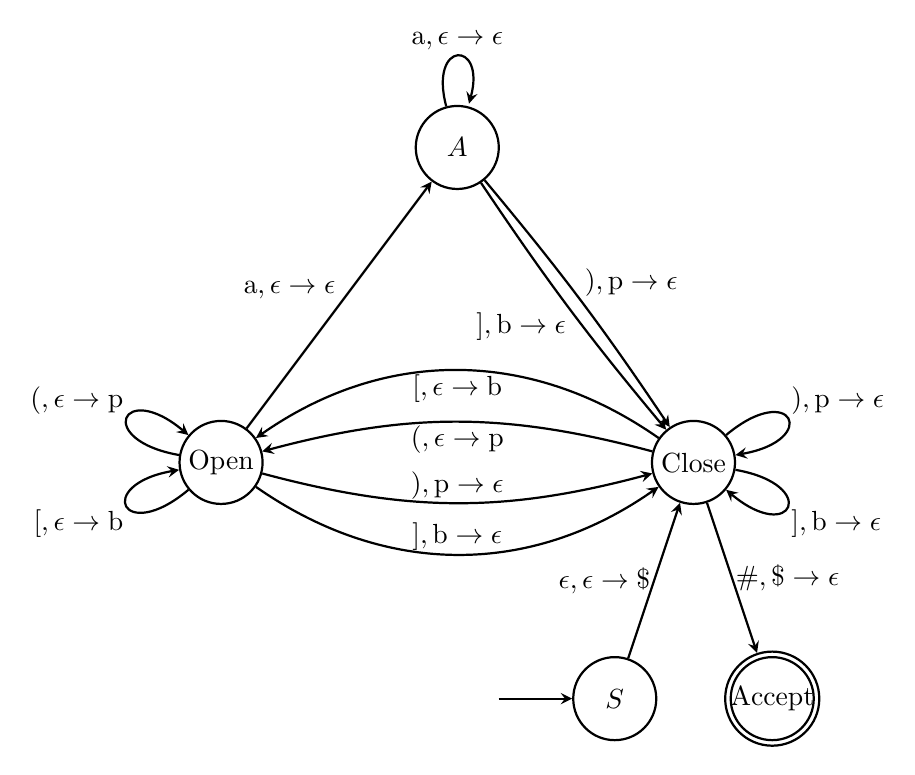
\begin{tikzpicture}
                \begin{scope}[auto, every node/.style={thick, draw,circle,minimum size=3em,inner sep=1}]
                        \node (S) at (5,0) {\(S\)};
                        \node (Op) at (0,3) {Open};
                        \node (A) at (3, 7) {\(A\)};
                        \node (Cl) at (6,3) {Close};
                        \node (Accept) at (7,0) {Accept};
                        \draw[black, thick] (7,0) circle [radius=1.5em];
                \end{scope}
                \node [draw=none, inner sep=0pt] (I) at (3.5,0) {};
                \begin{scope}[auto, every node/.style={minimum size=1em,inner sep=1}, every path/.style={thick, ->, >=stealth}]
                        \path (I) edge (S);
                        \path (S) edge node [left] {\(\epsilon, \epsilon\rightarrow\$\)} (Cl);
                        \path (Op) edge [loop,in=140,out=170,looseness=10] node {\(\text{(}, \epsilon\rightarrow\text{p}\)} (Op);
                        \path (Op) edge [loop,in=190,out=220,looseness=10] node {\(\text{[}, \epsilon\rightarrow\text{b}\)} (Op);
                        \path (Op) edge node {\(\text{a}, \epsilon\rightarrow\epsilon\)} (A);
                        \path (Op) edge [bend right=15] node {\(\text{)}, \text{p}\rightarrow\epsilon\)} (Cl);
                        \path (Op) edge [bend right=35] node {\(\text{]}, \text{b}\rightarrow\epsilon\)} (Cl);
                        \path (A) edge [loop above] node {\(\text{a}, \epsilon\rightarrow\epsilon\)} (A);
                        \path (A) edge [bend left=3] node {\(\text{)}, \text{p}\rightarrow\epsilon\)} (Cl);
                        \path (A) edge [bend right=3] node [below left] {\(\text{]}, \text{b}\rightarrow\epsilon\)} (Cl);
                        \path (Cl) edge [loop,in=10,out=40,looseness=10] node [above right] {\(\text{)}, \text{p}\rightarrow\epsilon\)} (Cl);
                        \path (Cl) edge [loop,in=320,out=350,looseness=10] node [below right] {\(\text{]}, \text{b}\rightarrow\epsilon\)} (Cl);
                        \path (Cl) edge [bend right=15] node {\(\text{(}, \epsilon\rightarrow\text{p}\)} (Op);
                        \path (Cl) edge [bend right=35] node {\(\text{[}, \epsilon\rightarrow\text{b}\)} (Op);
                        \path (Cl) edge node [right] {\(\text{\#}, \$\rightarrow\epsilon\)} (Accept);
                \end{scope}
        \end{tikzpicture}
\end{center}
Here is a deterministic pushdown automata with the stack symbols
\[\Gamma=\{\text{\#},\text{p},\text{b}\}\]
This is deterministic because for any combination of states, input symbols, and stack symbols, there is at most one move.
Unspecified transitions block, so for any input string this automata can only end up in a single state.

\section*{Problem 1}

\paragraph{a)}

\begin{center}
        \resizebox{\textwidth}{!}{
        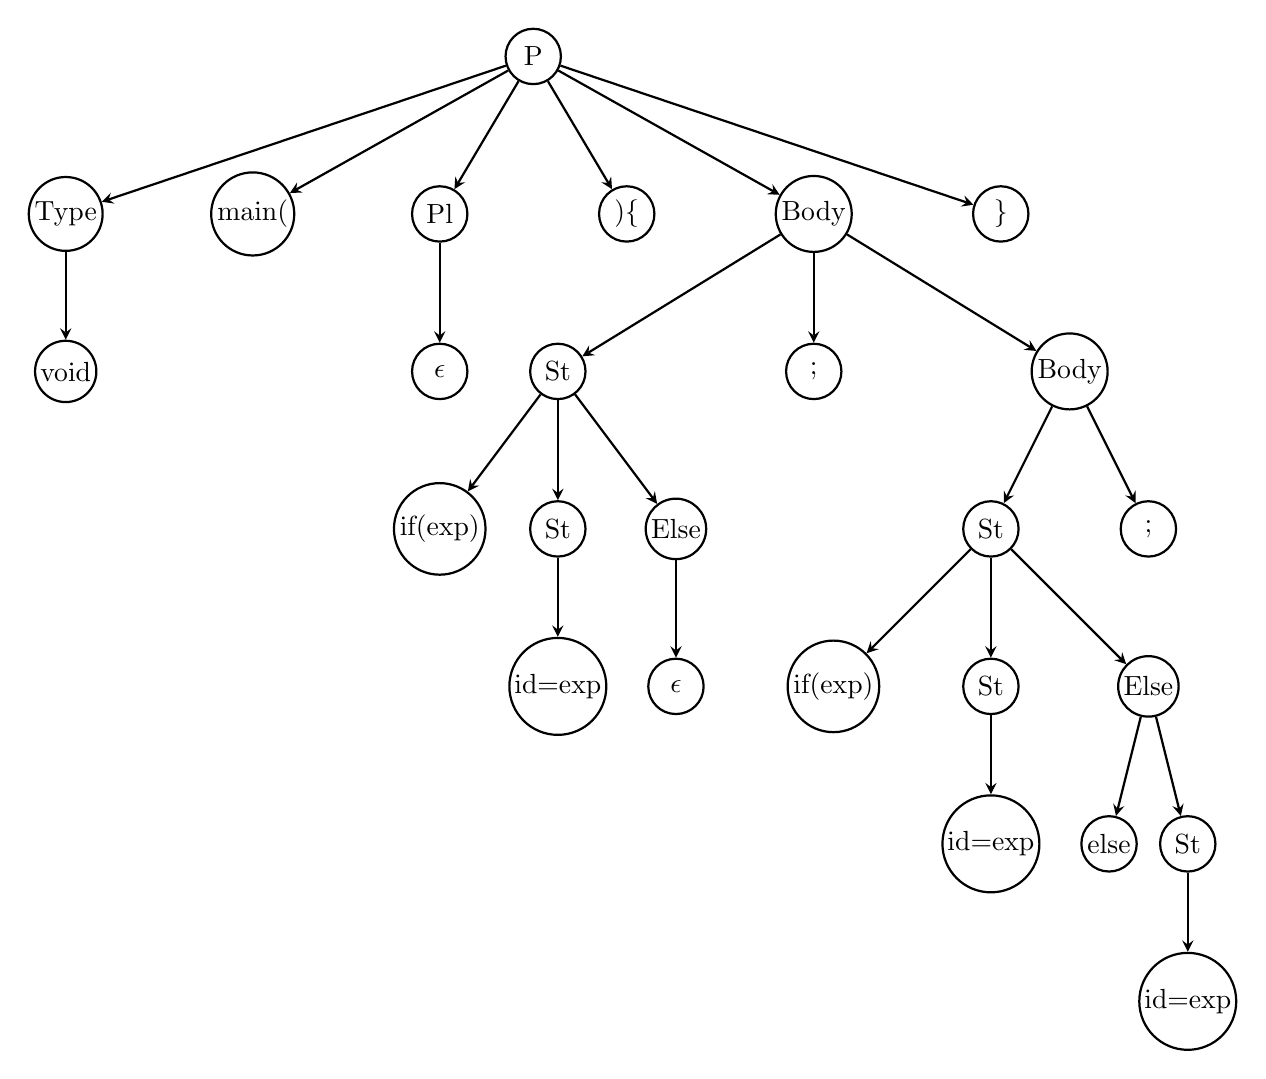
\begin{tikzpicture}
                \begin{scope}[auto, every node/.style={thick, draw,circle,minimum size=2em,inner sep=1}]
                        \node (P) at (5.9375,0) {P};
                        \node (Type) at (0,-2) {Type};
                        \node (Main) at (2.375,-2) {main(};
                        \node (Pl) at (4.75,-2) {Pl};
                        \node (Br1) at (7.125,-2) {)\{};
                        \node (Body1) at (9.50,-2) {Body};
                        \node (Br2) at (11.875,-2) {\}};
                        \node (Void) at (0,-4) {void};
                        \node (Ep1) at (4.75,-4) {\(\epsilon\)};
                        \node (St1) at (6.25,-4) {St};
                        \node (Col1) at (9.5,-4) {;};
                        \node (Body2) at (12.75,-4) {Body};
                        \node (If1) at (4.75,-6) {if(exp)};
                        \node (St2) at (6.25,-6) {St};
                        \node (Else1) at (7.75,-6) {Else};
                        \node (St3) at (11.75,-6) {St};
                        \node (Col2) at (13.75,-6) {;};
                        \node (Id1) at (6.25,-8) {id=exp};
                        \node (Ep2) at (7.75,-8) {\(\epsilon\)};
                        \node (If2) at (9.75,-8) {if(exp)};
                        \node (St4) at (11.75,-8) {St};
                        \node (Else2) at (13.75,-8) {Else};
                        \node (Id2) at (11.75,-10) {id=exp};
                        \node (TElse) at (13.25,-10) {else};
                        \node (St5) at (14.25,-10) {St};
                        \node (Id3) at (14.25,-12) {id=exp};
                \end{scope}
                \begin{scope}[auto, every node/.style={minimum size=1em,inner sep=1}, every path/.style={thick, ->, >=stealth}]
                        \path (P) edge (Type);
                        \path (P) edge (Main);
                        \path (P) edge (Pl);
                        \path (P) edge (Br1);
                        \path (P) edge (Body1);
                        \path (P) edge (Br2);
                        \path (Type) edge (Void);
                        \path (Pl) edge (Ep1);
                        \path (Body1) edge (St1);
                        \path (Body1) edge (Col1);
                        \path (Body1) edge (Body2);
                        \path (St1) edge (If1);
                        \path (St1) edge (St2);
                        \path (St1) edge (Else1);
                        \path (Body2) edge (St3);
                        \path (Body2) edge (Col2);
                        \path (St2) edge (Id1);
                        \path (Else1) edge (Ep2);
                        \path (St3) edge (If2);
                        \path (St3) edge (St4);
                        \path (St3) edge (Else2);
                        \path (St4) edge (Id2);
                        \path (Else2) edge (TElse);
                        \path (Else2) edge (St5);
                        \path (St5) edge (Id3);
                \end{scope}
        \end{tikzpicture}
        }
\end{center}

\paragraph{b)}
\begin{center}
\underline{void}main()\{if(exp)id=exp;if(exp)id=expelseid=exp;\}\\
Typemain(\underline{\(\epsilon\)})\{if(exp)id=exp;if(exp)id=expelseid=exp;\}\\
Typemain(Pl)\{if(exp)\underline{id=exp};if(exp)id=expelseid=exp;\}\\
Typemain(Pl)\{if(exp)St\underline{\(\epsilon\)};if(exp)id=expelseid=exp;\}\\
Typemain(Pl)\{\underline{if(exp)StElse};if(exp)id=expelseid=exp;\}\\
Typemain(Pl)\{St;if(exp)\underline{id=exp}elseid=exp;\}\\
Typemain(Pl)\{St;if(exp)Stelse\underline{id=exp};\}\\
Typemain(Pl)\{St;if(exp)St\underline{elseSt};\}\\
Typemain(Pl)\{St;\underline{if(exp)StElse};\}\\
Typemain(Pl)\{St;\underline{St;}\}\\
Typemain(Pl)\{\underline{St;Body}\}\\
\underline{Typemain(Pl)\{Body\}}\\
P
\end{center}

\paragraph{c)}

The only language features that require the CFG model are the statement and else features. This is because
they can be nested to create infinite pairs of matching curly braces. The other language features only require
DFA's because they are either in a fixed format like the overall structure and the finite type list, or they are
an infinite list that doesn't require matching like the parameter list and body statement. Thus only the statement
and else features require the CFG model since they create infinite nested matching.

\section*{Problem 2}

Assume for contradiction that \(L_2\) is a context free language. Then by the pumping lemma for context free languages
there exists some \(p\) such that for any string \(s\in L_2\) with length greater than \(p\), the string \(s\) can be
split into five substrings \(u\), \(v\), \(w\), \(x\), and \(y\) such that \(s=uvwxy\), \(|vwx|\leq p\), \(|vx|>0\), and
\(\forall i\geq 0\) we have that \(uv^iwx^iy\in L_2\). But consider the string \(s=0^p10^{p+1}10^p\) which is in \(L_2\). When
attempting to split \(s\) into five substrings to satisfy the puming lemma, we have that \(vwx\) can contain either one or zero
1's, since the two 1's are more than \(p\) characters apart.

If \(vwx\) contains zero 1's, then \(vx\) must consist entirely of zeroes, and both \(v\) and \(x\) lie either before the
first 1, between the two 1's, or after the second 1. If both \(v\) and \(x\) lie before the first 1, the string \(uv^iwx^iy\)
will not be in \(L_2\) since for \(i>2\) the string will take the form \(0^r10^{p+1}10^p\) with \(r\geq p+1\). If both \(v\)
and \(x\) lie between the two 1's, the string \(uv^iwx^iy\) will not be in \(L_2\) since for \(i=0\) the string will take
the form \(0^p10^r10^p\) with \(r\leq p\). If both \(v\) and \(x\) lie after the second 1, the string \(uv^iwx^iy\) will
not be in \(L_2\) since for \(i>2\) the string will take the form \(0^p10^{p+1}10^r\) with \(r\geq p+1\). So \(vwx\) cannot contain
zero 1's.

If \(vwx\) contains one 1, then \(vx\) must either contain one or zero 1's. If \(vx\) contains one 1, then the string \(uv^iwx^iy\)
will not be in \(L_2\) since for \(i>2\) the string will contain at least three 1's. \(L_2\) only includes strings with exactly two 1's.
If \(vx\) contains zero 1's and \(vwx\) contains one 1, then \(w\) contains one 1 and \(v\) and \(x\) must consist entirely of 0's. Additionally,
either \(v\) lies before the first 1 and \(x\) lies in between the two 1's, or \(v\) lies between the two 1's and \(x\) lies after the second 1.
If \(v\) lies before the first 1 and \(x\) lies in between the two 1's, we have that \(|v|\leq |x|\), since if \(|v|>|x|\) the string \(uv^iwx^iy\)
would have the form \(0^r10^s10^p\) with \(r\geq s\) for \(i>2\), which is not in \(L_2\). Because \(|vx|>0\), this means that \(|x|>0\). But if \(|x|>0\),
the string \(uv^iwx^iy\) would have the form \(0^r10^s10^p\) with \(p\geq s\) for \(i=0\), so the string would not be in \(L_2\).
So \(v\) cannot lie before the first 1 while \(x\) lies in between the two 1's. If \(v\) lies between the two 1's and \(x\) lies after the second 1,
we have that \(|x|\leq |v|\), since if \(|x|>|v|\) the string \(uv^iwx^iy\) would have the form \(0^p10^s10^r\) with \(r\geq s\) for \(i>2\), which is not in \(L_2\).
Because \(|vx|>0\), this means that \(|v|>0\). But if \(|v|>0\), the string \(uv^iwx^iy\) would have the form \(0^p10^s10^r\)
with \(p\geq s\) for \(i=0\), so the string would not be in \(L_2\). So \(vwx\) cannot contain one 1, and there is no valid way to
split \(s\) into five substrings such that the pumping lemma holds. This is a contradiction, and thus \(L_2\) is not a context free language.

\end{document}